\documentclass[submission,copyright,creativecommons]{eptcs}
\usepackage{breakurl}             % Not needed if you use pdflatex only.
\usepackage{datetime}
\newdate{date}{04}{18}{2018}
%\date{\displaydate{date}}
\usepackage{graphicx} %package to manage images
\graphicspath{ {images/} }

\usepackage[rightcaption]{sidecap}

\usepackage{wrapfig}
\title{Blockchain principles applied to transaction operations on the Real Estate Market}
\author{Andres Salgado
\institute{International Technological University\\ San Jose, California, \underline{USA}}
\email{salgadoandre533@students.itu.edu}
\and
Co Authors \qquad\qquad Jorge Valdeiglesias, Kartikeya Yellayi
\institute{International Technological University\\ San Jose, California, \underline{USA}}
\email{\quad valdeiglesjorge744@students.itu.edu \quad\qquad yellayishiva1284@students.itu.edu}
}

\def\titlerunning{Blockchain principles applied to transaction operations on the Real Estate Market}
\def\authorrunning{Andres Salgado, C. Author \& Jorge Valdeiglesias, Kartikeya Yellayi}

\begin{document}
\maketitle
\displaydate{today}

\begin{abstract}
This is a sentence in the abstract.
This is another sentence in the abstract.
This is yet another sentence in the abstract.
This is the final sentence in the abstract.
\end{abstract}

\section{Introduction}

With the advent of ``blockchain'' technologies, as well as the necessity to establish a system where the trust of transactions could be offloaded to machines, we ventured into exploring how a system based on the Ethereum blockchain could accurately execute a series of smart contracts in order to validate a transaction between two entities.

%By means of the style-file option
%\href{http://creativecommons.org/about/license/}{creativecommons}
%authors equip their paper with a Creative Commons license that allows
%everyone to copy, distribute, display, and perform their copyrighted
%work and derivative works based upon it, but only if they give credit%the way you request. By invoking the additional style-file option {\tt
%noderivs} you let others copy, distribute, display, and perform only
%verbatim copies of your work, but not derivative works based upon
%it. Alternatively, the {\tt sharealike} option allows others to
%distribute derivative works only under a license identical to the
%license that governs your work. Finally, you can invoke the option
%{\tt noncommercial} that let others copy, distribute, display, and
%perform your work and derivative works based upon it for
%noncommercial purposes only.


\section{The blockchain and its influence on crypto-currencies}

It's close to 10 years after Bitcoin was introduced by Satoshi Nakamoto. The reason crypto-currencies currently exist is due to the underlying technology made available by the blockchain. Thomas Lowenthal from Ars Technica \cite{lowenthalBitcoinEncryptedPeertopeer2011} goes onto explaining the complexities of cryptographic currencies, the concept of mining and make-work, and goes onto comparing Bitcoin against the trusty greenback which also faced hurdles when it was first put into circulation.

The primary reason why cryptocurrencies are being adopted by a sizable portion of the population is due to the engineering concept behind the implementation of the blockchain to solve two basic problems inherent to digital currencies, the double-spending problem, and the prevention of counterfeiting\cite{noauthor_bitcoin}.
On cppcon 2016 David Schwarz\cite{cppconCppCon2016David} at cppcon 2016 spoke about "Developing Blockchain Software".  On his talk he mentions key characteristics of "the blockchain". Section 2.1 goes onto describing such characteristics.   

\subsection{What is a blockchain and what is one good for?}
\begin{itemize}
\item Blockchains record state and history
\item State is modified by transactions
\item Everyone eventually agrees on the transactions
\item Can be used to transfer tokens
\end{itemize}

Based on this list, most of us would conclude that the blockchain is merely a database, but in actuality, the blockchain -according to Schwarz\cite{cppconCppCon2016David}- manages the double-spending problem.

\subsection{What the blockchain does for bitcoin}

Figure 1 describes how the blockchain validates bitcoin as cryptocurrency system\cite{noauthor_bitcoin}
\begin{figure}[h]
    \centering
    \label{fig:my_label}
    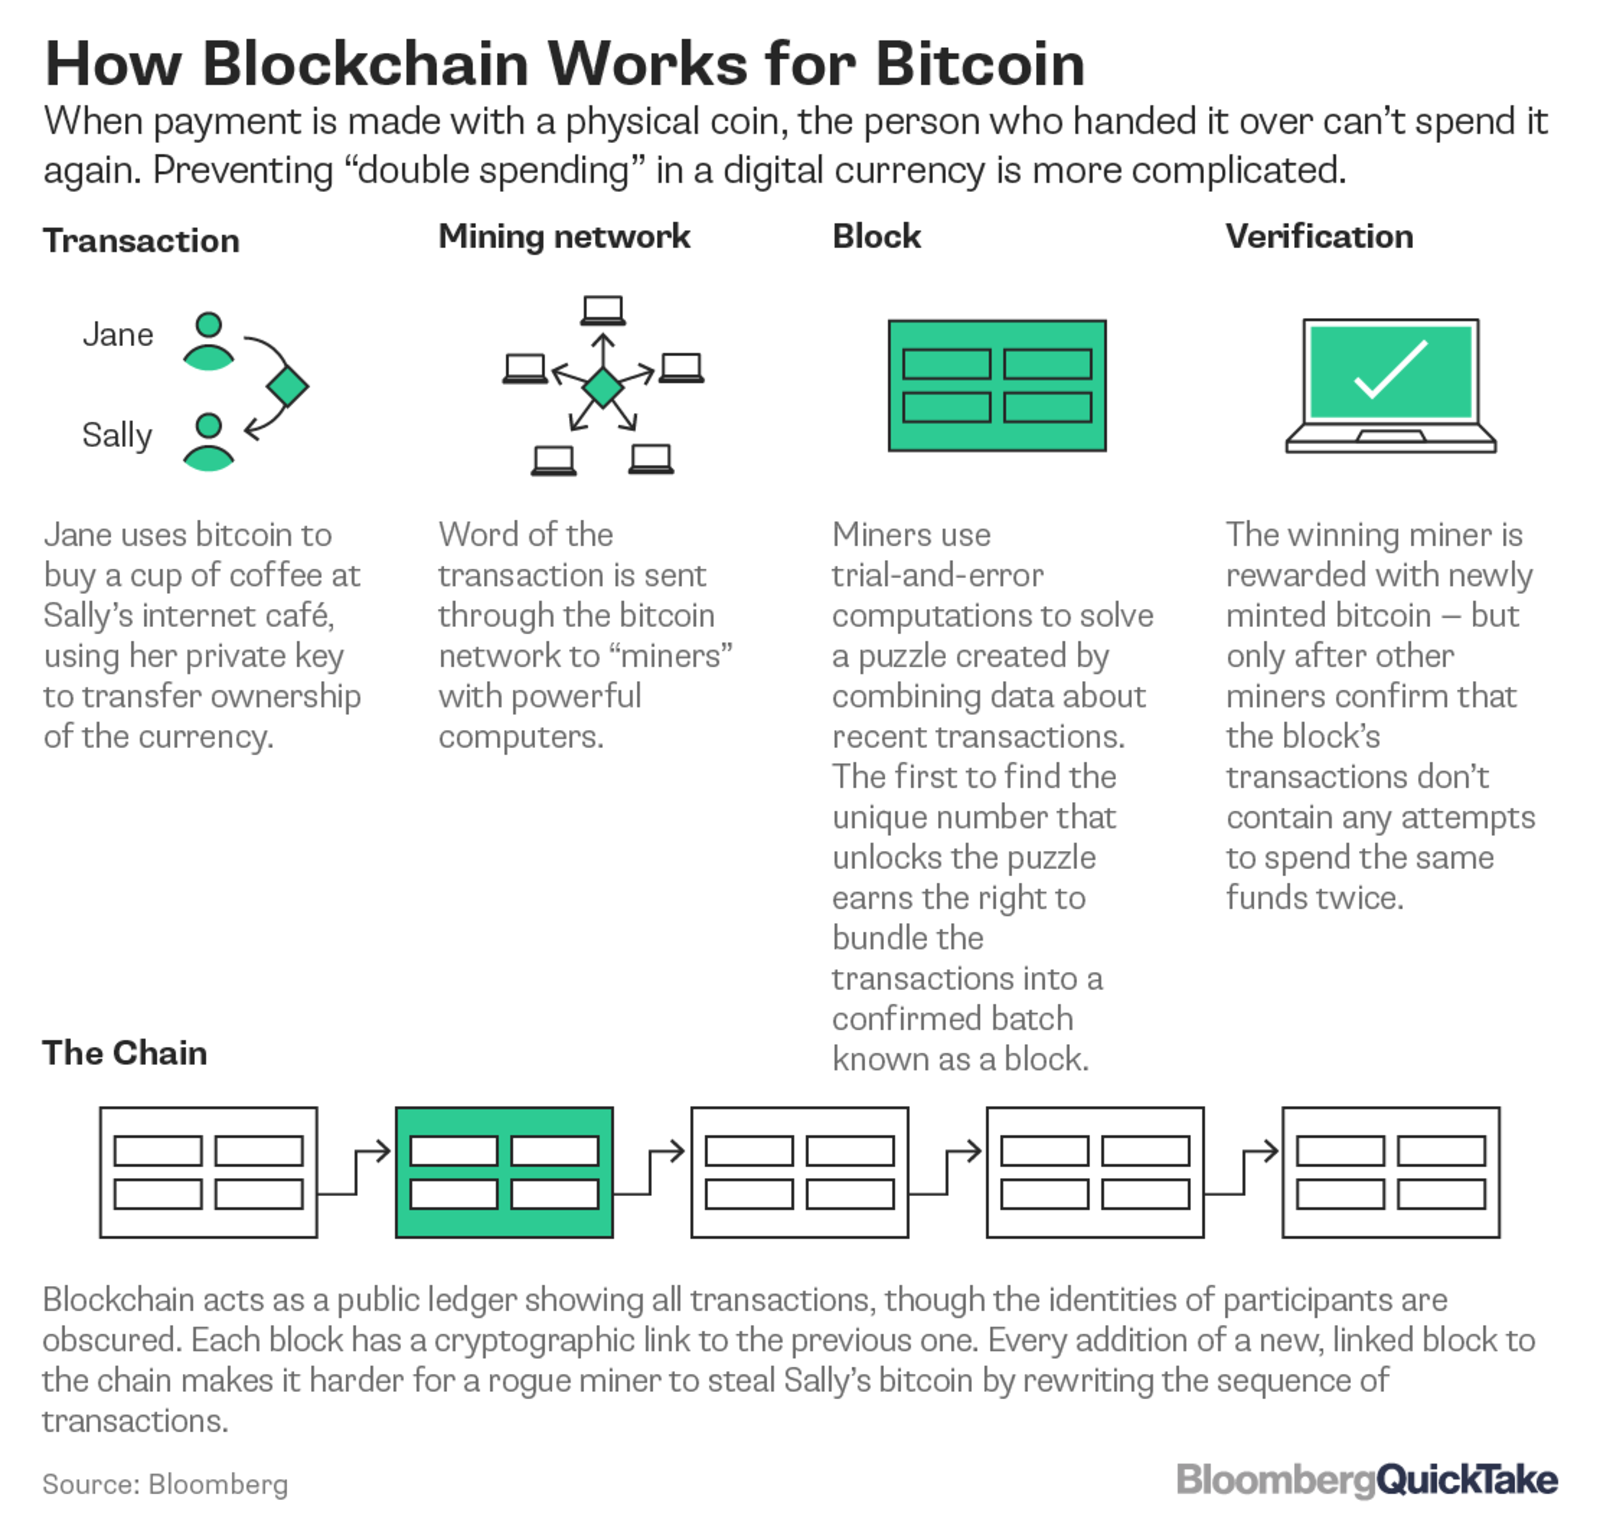
\includegraphics[width=5in]{bitcoin-blockchain-bloomberg}
     \caption{Image Source: BloombergQuicktake}
\end{figure}.

\subsection{Principal advantages of cryptocurrencies}
Not only does Bitcoin comply with providing security to users that require to exchange currency within the system, but by December 2017\cite{MostImportantCryptocurrencies} the 6 most important cryptocurrencies in world, among those \textit{Ethereum} which is currently the second cryptocurrency based on market capitalization \textbf{(41.4 billion)}, manage to .

\section{Beyond Bitcoin (other industries and its use)}
Besides solving the issue of how to allow for a feasible digital currency, the blockchain has opened the door towards the development of new uses of the technology, that do not necessarily address the exchange of assets in a digital manner.  This exposure has allowed millions of dollars to be poured into research and development of proper blockchain applications in a variety of fields with distinct uses and outcomes.
One of the business that seems to be benefiting the most from this investments is the logistics business. Many companies are involved in the process of carrying goods. Most importantly, because there are several actors involved in such process, a delay in shipment can prove to be catastrophic to huge shipments.  

Currently the majority of companies that engage in gathering data to make business decisions use different types of database systems in order to store, query and build statistical models out of collected data.  When the interaction with that data doesn't require sharing such information, companies are equipped to process it, but when two or more entities\cite{BlockchainGoesCryptoCurrency2016} need to share such data, it is often complicated to achieve a consensus on how such exchange should be handled.\footnote{Olga Kharif on her article "Blockchain Goes Beyond Crypto-Currency" explains how companies in Finland, Sweden, Estonia and Latvia are beginning to use a blockchain system in order to share information.}

\section{Ethereum and smart contracts}
Back in 1996, Nick Szabo\footnote{Nick Szabo is credited as one of the first proponents of the us of smart contracts on the digital realm.} layed much of the ground work of what we currently know as \textit{"Smart Contracts"}.  On \textit{"Smart Contracts: Building Blocks for Digital Markets"}\cite{NickSzaboSmart} Szabo makes a conspicuous argument on how our society has built a structure based on the common law of contracts.  He\footnote{Szabo does a marvelous job on explaining how our society arrived to the use of contracts and how these contracts are the bedrock of a free market economy.} is meticulous when explaining the role that contracts play into our current free market economy.  The article's introduction does not try to impose digital contracts as a replacement to our current system of values and the concept of agreements and contracts, but instead opens the door to a discourse on how computers in a digital society can improve or aid towards making the then current system more functional.

Many experts conclude that \textit{Bitcoin} has done to the blockchain what e-mail did to the internet.  To further this notion of what the blockchain is capable of, it can be said that \textit{Bitcoin} is a digital currency using the blockchain as a vehicle to function digitally.  There are certain tasks that \textit{Bitcoin} can perform, but they are limited compared to that of the scope of what \textit{Ethereum} does.  One of the main advantages of \textit{Ethereum} is that it applies the same principles that the blockchain uses on \textit{Bitcoin} with the added functionality of smart contracts\footnote{Smart contracts are currently handled by the Solidity language.  Further information about solidity can be found at the development website \url{https://solidity.readthedocs.io/en/develop/#}\cite{SoliditySolidity23}} as a method to exchange any item of value, this being money, content, shares or property.

Due to the advantages that \textit{Ethereum} offers we chose to dig a little deeper into finding a a set of tools that would allow our app to thrive towards developing a self-serving real estate property exchange tool.

\subsection{RSA silently working on the background}
Szabo puts great emphasis on explaining the background of RSA\cite{milanov2009rsa} and its critical role on smart contracts.  The ideal metaphor uses two subjects -in this case Alice and Bob- to explain how public cryptography's mathematical intricacies work to create a pair of \textit{keys} in this case a public one and private one that serve as a cryptography based exchange of messages.  The importance of the use of RSA based encryption is directly related to the underpinning of the principles of contract design\footnote{Szabo goes on to explaining these principles on the \textit{Some Basic Principles of Contract Design} subsection of \cite{NickSzaboSmart}} and are rooted on common law, economic theory, and contractual conditions, which in turn derive the principles of observability, verifiability, privity, and enforceability.



\subsection{Smart Contract definition}
An abridged definition of the smart contract provided by the \textit{Solidity} documentation page goes as follows:
\begin{quote}
    A contract in the sense of Solidity is a collection of code (its functions) and data (its state) that resides at a specific address on the Ethereum blockchain.\cite{IntroductionSmartContracts}
\end{quote}
In a strict technical sense, the smart contract is programmable to comply with any set of defined conditions.  Because the smart contract is rooted in code, any prerequisite that was celebrated between two parties on a traditional contract, can have its clauses translated into code, therefore allowing for any legal conditions to exist digitally.

\textit{Figure 2} illustrates how a smart contract would execute the sale of a property.  In this case two parties, the buyer and the seller, \textbf{exchange} an asset through a contract that supports the digitizing of a land deed and the subsequent digitizing of the currency, allowing for an ordered settlement and thus cementing the idea that the ownership of the asset was properly transferred to the new owner\cite{WhatAreSmart}.
\begin{figure}[h]
    \centering
    \label{fig:howsmartcontractsworks}
    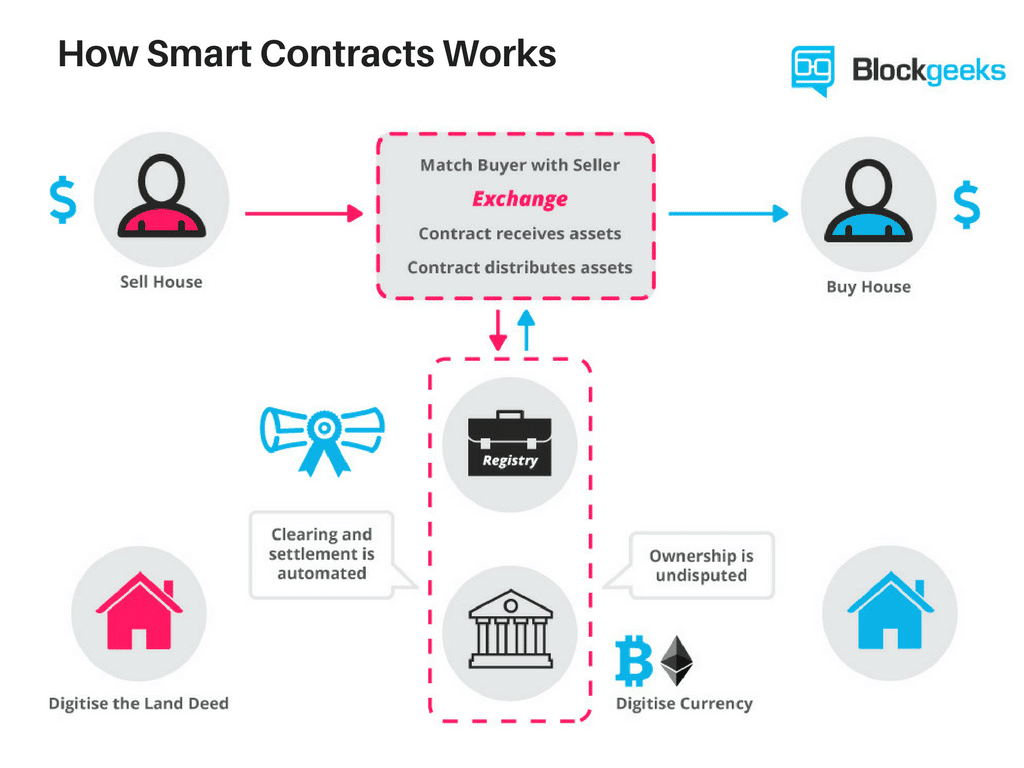
\includegraphics[width=5in]{How-Smart-Contracts-Works-1.png}
     \caption{Image Source: Blockgeeks}
\end{figure}

\subsection{Zeroing on Ethereum}
\textit{Ethereum's} versatility, served as the perfect platform to deploy a generalized decentralized app seeking to solve smart contract transactions.  Dr. Gavin Wood in his introduction to \textit{ETHEREUM: A SECURE DECENTRALISED GENERALISED TRANSACTION LEDGER} summarizes the objectives of building \textit{"a trustful object messaging compute framework."}\cite{wood2014ethereum}Parting from these principles the platform choice selected for accomplishing the objective of our thesis revolves around the use of a framework grounded on \textit{Ethereum}. 

Research concluded that the chosen framework needed to have current front-end and back-end technologies, as well as to show signs of current community engagement and active development.  

\section{Truffle as a development platform}
\textit{Truffle} is a Javascript based development framework\cite{TruffleDocumentation}. \textit{Truffle} offers the following advantages as a tool:
\begin{itemize}
\item Built-in smart contract compilation, linking, deployment and binary management.
\item Automated contract testing for rapid development.
\item Scriptable, extensible deployment & migrations framework.
\item Network management for deploying to any number of public & private networks.
\item Package management with EthPM & NPM, using the ERC190 standard.
\item Interactive console for direct contract communication.
\item Configurable build pipeline with support for tight integration.
\item External script runner that executes scripts within a Truffle environment.
\end{itemize}

In order to deploy and test the validity and accuracy of the contracts written within our coding environment, it was necessary to write the contracts to a blockchain.  The creators of \textit{Truffle} simultaneously develop and maintain a separate component named \textit{Ganache}.  \textit{Ganache}\cite{Ganache} is a personal deployable test Ethereum network capable of accepting commands, with a GUI interface that allows users to inspect and control how the chain operates.  It is a requirement for Ganache to run in the background in order to properly test the validity and actionability of any given contract code written in the application.


\newpage
\section{Bibliography}




\bibliographystyle{acm}
\bibliography{biblio}
%\listoffigures
\end{document}
